\documentclass[12pt, a4paper]{article}\usepackage{listings}
\usepackage{hyperref}
\usepackage{amsmath}
\usepackage {graphicx}	
\usepackage{geometry}	% Ermöglicht das ändern der Seitenränder

\geometry{
	left = 3.15cm, % Normaler Seitenabstand Lniks
	right = 3.15cm % Normaler Seitenabstand Rechts
}

\title{VPCS Konfigurationsanleitung in GNS3}
\author{Lukas Köppl}
\date{\today}

\begin{document}

\maketitle
\newpage
\tableofcontents
\newpage

\section{Übung: Anleitung zur Konfiguration eines VPCS in GNS3}

\subsection{Ziehe einen VPCS in den Workspace}
\begin{itemize}
    \item Öffne die GNS3-Anwendung.
    \item Klicke im linken Gerätefenster auf \textbf{VPCS}.
    \item Ziehe das \textbf{VPCS}-Symbol in den zentralen Workspace.
\end{itemize}

\subsection{Ändere den Namen auf \texttt{MeinVPCS}}
\begin{itemize}
    \item Klicke mit der rechten Maustaste auf das VPCS-Icon im Workspace.
    \item Wähle \textbf{Umbenennen} oder \textbf{Rename}.
    \item Gib den neuen Namen \texttt{MeinVPCS} ein und bestätige.
\end{itemize}

\subsection{Ändere die Einstellungen, sodass die Konsole automatisch startet}
\begin{itemize}
    \item Klicke mit der rechten Maustaste auf das VPCS-Symbol im Workspace.
    \item Wähle \textbf{Einstellungen} oder \textbf{Settings}.
    \item Gehe zum Bereich \textbf{Konsole} oder \textbf{Console settings}.
    \item Suche nach der Option \textbf{Automatisch starten} oder \textbf{Auto start console}.
    \item Aktiviere diese Option und klicke auf \textbf{Übernehmen} oder \textbf{Speichern}.
\end{itemize}

\subsection{Starte das System}
\begin{itemize}
    \item Klicke mit der rechten Maustaste auf das VPCS und wähle \textbf{Start}.
    \item Die Konsole sollte automatisch starten, wenn alles korrekt eingestellt wurde.
\end{itemize}

\subsection{Hilfe anzeigen mit \texttt{?}}
\begin{itemize}
    \item Sobald die Konsole gestartet ist, gib \texttt{?} ein und drücke \texttt{Enter}.
    \item Eine Liste der verfügbaren VPCS-Befehle und deren Beschreibungen wird angezeigt.
\end{itemize}

\subsection{Setze die IP-Adresse auf \texttt{192.168.3.2/24}}
\begin{itemize}
    \item In der VPCS-Konsole gib den folgenden Befehl ein:
    \begin{verbatim}
ip 192.168.3.2 255.255.255.0
    \end{verbatim}
    \item Drücke \texttt{Enter}, um die IP-Adresse zu setzen.
\end{itemize}

\subsection{IP-Adresse anzeigen}
\begin{itemize}
    \item Um die IP-Adresse zu überprüfen, gib den folgenden Befehl ein:
    \begin{verbatim}
show ip
    \end{verbatim}
    \item Die aktuelle IP-Adresse und Subnetzmaske werden angezeigt.
\end{itemize}

\subsection{Einstellungen der Maschine speichern}
\begin{itemize}
    \item Gib den folgenden Befehl ein, um die Konfiguration zu speichern:
    \begin{verbatim}
save
    \end{verbatim}
    \item Die Einstellungen werden gespeichert und bleiben beim nächsten Start erhalten.
\end{itemize}

\newpage

\section{Übung: VPC1 auf VPC2 pingen}
\begin{itemize}
	\item Füge zwei VPCs wie in Übung 1 in deine Workspace
	\item Ändere deren IP Adressen auf 192.168.3.{2,3} mit:
		\begin{verbatim}
ip 192.168.3.2 255.255.255.0
		\end{verbatim}
	\item Lass dir die IPs der Systeme anzeigen mit:
		\begin{verbatim} 
show ip 
		\end{verbatim}
	\item Speichere die Einstellungen der Maschine mit:
		\begin{verbatim} 
save 
		\end{verbatim}			
	\item Verbinde die beiden Maschinen mit einem Netzwerkkabel jeweils auf Port0
	\item Versuch mittels ping zu überprüfen ob die Maschinen verbunden sind mit:
		\begin{verbatim}
ping 192.168.3.2 (Beispiel IP)
		\end{verbatim}
\end{itemize}

\newpage

\section{Übung: Hub und Switch}
\textbf{Connection:} \quad \textbf{IP-Adressen:}
\begin{itemize}
  \item PC1.Ethernet0 mit Hub1.Ethernet0 \quad PC1 192.168.3.2
  \item PC2.Ethernet0 mit Hub1.Ethernet1 \quad PC2 192.168.3.3
  \item PC3.Ethernet0 mit Hub1.Ethernet2 \quad PC3 192.168.3.4
\end{itemize}
\subsection{Hub}
\subsubsection{Wireshark Analyse}
\begin{figure}[hbtp]
	\centering
	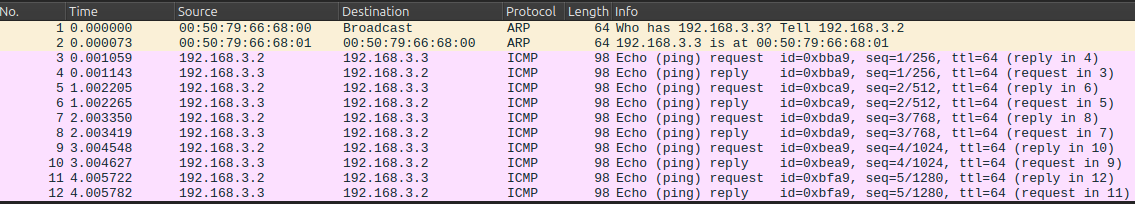
\includegraphics[width=1\textwidth]{images/Wireshark_Ping_HUB.png}
	\caption{Wireshark Analyse mit 3VPCs und 1Hub}
	\label{fig:HUB-Analyse}
\end{figure}

\begin{itemize}
    \item \textbf{Zeile 1:} ARP Anfrage: Gerät mit MAC-Adresse 00:50:79:66:68:00 (192.168.3.2) fragt nach der MAC-Adresse von 192.168.3.3.
    \item \textbf{Zeile 2:} ARP Antwort: Gerät 192.168.3.3 antwortet mit MAC-Adresse 00:50:79:66:68:01.
    \item \textbf{Zeilen 3 bis 12:} ICMP Echo-Anfragen und -Antworten (Ping):
    \begin{itemize}
        \item \textbf{Zeile 3:} 192.168.3.2 sendet Ping-Anfrage an 192.168.3.3 (ID=0xbba9, Seq=1/256).
        \item \textbf{Zeile 4:} 192.168.3.3 antwortet mit Ping-Antwort.
        \item Dieser Vorgang wiederholt sich für weitere Ping-Anfragen (ID=0xbca9, 0xbda9, 0xbea9, 0xbfa9) und Antworten.
    \end{itemize}
\end{itemize}

\newpage

\subsection{Switch}
\subsubsection{Wireshark Analyse}
\begin{figure}[hbtp]
	\centering
	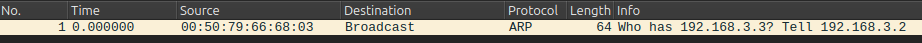
\includegraphics[width=1\textwidth]{images/Wireshark_Ping_Switch.png}
	\caption{Wireshark Analyse mit 3VPCs und 1Swich}
	\label{fig:HUB-Analyse}
\end{figure}
\begin{itemize}
    \item \textbf{Zeile 1: ARP Anfrage:}  
    Das Gerät mit der MAC-Adresse 00:50:79:66:68:03 (IP: 192.168.3.2) sendet eine ARP-Anfrage als Broadcast, um die MAC-Adresse von 192.168.3.3 zu ermitteln. Die Anfrage wird an alle Geräte im Subnetz weitergeleitet, da der Switch keine Informationen über die MAC-Adressen in der Kommunikation hat.
\end{itemize}

\subsection{Was hat sich geändert und warum?}
\begin{itemize}
    \item Der **Hub** sendet alle Daten an alle Geräte, was zu unnötigem Verkehr und mehr Kollisionen führt. Dies ist ineffizient und kann die Netzwerkgeschwindigkeit verringern.
    \item Der **Switch** hingegen filtert den Verkehr und leitet Daten nur an das Zielgerät weiter. Dadurch wird der Datenverkehr optimiert, und die Wahrscheinlichkeit von Kollisionen wird verringert.
    \item Die Änderung vom Hub zum Switch führt zu einer signifikanten Verbesserung der Netzwerkleistung, da der Switch intelligenter und effizienter mit den Datenströmen umgeht.
\end{itemize}

\newpage
\section{Übung: Erstelle ein neues Projekt und konfiguriere einen OpenWrt Router}

\subsection{Erstelle ein neues Projekt}
\begin{itemize}
    \item Öffne die GNS3-Anwendung.
    \item Klicke auf \textbf{Datei → Neues Projekt} oder \textbf{File → New Project}.
    \item Gib deinem Projekt einen passenden Namen (z.\,B. \texttt{OpenWrt-Router}).
    \item Wähle den Speicherort und klicke auf \textbf{OK}.
\end{itemize}

\subsection{Erstelle ein neues Router-Template}
\begin{itemize}
    \item Gehe zu \textbf{Router → New template}.
    \item Wähle \textbf{Install an appliance from the GNS3 server (recommended)} und klicke auf \textbf{Next}.
    \item Suche nach \textbf{OpenWrt} und wähle die entsprechende Option aus.
    \item Klicke auf \textbf{Install → Install the appliance on the GNS3 VM (recommended)} oder \textbf{Install the appliance on your local computer}, je nachdem, wo du GNS3 ausführst.
\end{itemize}

\subsection{OpenWrt herunterladen und konfigurieren}
\begin{itemize}
    \item Wähle die \textbf{OpenWrt version 23.05.05} aus.
    \item Lade die Datei \texttt{openwrt-23.05.5-x86-64-combined-ext4.img} herunter.
    \item Kopiere die heruntergeladene Datei in das Verzeichnis \texttt{GNS3/images/QEMU}.
    \item Entpacke die Datei mit folgendem Befehl im Terminal:
    \begin{verbatim}
gunzip openwrt-23.05.5-x86-64-combined-ext4.img.gz
    \end{verbatim}
    \item Aktualisiere die Liste der verfügbaren Images in GNS3, indem du auf \textbf{Refresh} klickst.
    \item Wähle das entpackte Image aus, klicke auf \textbf{Next}, und bestätige die Installation.
\end{itemize}

\subsection{Füge den Router und eine NAT-Node zum Workspace hinzu}
\begin{itemize}
    \item Ziehe den neu erstellten OpenWrt-Router in den Workspace.
    \item Ziehe eine \textbf{NAT Node} in den Workspace.
    \item Verbinde \textbf{openwrt-23.05.5-1.Ethernet1} mit \textbf{NAT1.Ethernet0}.
\end{itemize}

\subsection{Starte den Router und öffne die Konsole}
\begin{itemize}
    \item Starte den Router, indem du mit der rechten Maustaste darauf klickst und \textbf{Start} auswählst.
    \item Öffne die Konsole des Routers.
\end{itemize}

\subsection{Verschaffe dir einen Überblick über die IPv4-Konfiguration}
\begin{itemize}
    \item In der Router-Konsole gib den folgenden Befehl ein:
    \begin{verbatim}
ip -4 addr show
    \end{verbatim}
    \item Die aktuelle IPv4-Konfiguration des Routers wird angezeigt.
\end{itemize}

\subsection{Beschreibung und Begründung der IPv4-Konfiguration}
\begin{itemize}
    \item Die Ausgabe zeigt die IPv4-Adressen der Schnittstellen des Routers.
    \item \textbf{Beispiel:} Die Schnittstelle \texttt{eth1} (mit NAT verbunden) erhält durch den NAT-Node automatisch eine IPv4-Adresse, beispielsweise \texttt{10.0.2.15/24}.
    \item \textbf{Grund:} Der NAT-Node stellt ein Gateway bereit, das Adressinformationen automatisch über DHCP an verbundene Geräte vergibt. Der Router ist so mit dem Internet verbunden.
    \item Die andere Schnittstelle (z.\,B. \texttt{eth0}) ist standardmäßig ohne zugewiesene Adresse und kann manuell konfiguriert werden.
\end{itemize}

\newpage
\newpage
\subsection{Ändern der IP-Adresse des Routers}

Um die IP-Adresse des Routers von \texttt{br-lan} auf \texttt{192.168.3.1/24} zu ändern, gehe folgendermaßen vor:

\begin{enumerate}
    \item Logge dich in OpenWrt ein.
    \item Ändere die IP-Adresse des \texttt{br-lan} Interfaces mit:
    \begin{itemize}
    \item Öffne die Config Files des Netzwerk: (in der Router Konsole
    \begin{verbatim}
vi /etc/config/network
    \end{verbatim}
    \item Ändere die Config-File um folgende Zahlen um, die IP des Routers zu ändern, zwei weitere Ports freizuschalten und den router als Switch zu benutzen.
        \begin{verbatim}
config device
        option name 'br-lan'
        option type 'bridge'
        list ports 'eth0'
        list ports 'eth2'
        list ports 'eth3'

config interface 'lan'
        option device 'br-lan'
        option proto 'static'
        option ipaddr '192.168.3.1'
        option netmask '255.255.255.0'
        option ip6assign '60'
    \end{verbatim}
    \item resatart und reload die jeweiligen Config-Files
\begin{verbatim}
/etc/init.d/network restart
/etc/init.d/network reload
\end{verbatim}
    \end{itemize}
\end{enumerate}

\newpage

\subsection{Was bedeutet \texttt{/24}?}

Die Endung \texttt{/24} bezeichnet die Subnetzmaske und bedeutet, dass die ersten 24 Bits der IP-Adresse für das Netzwerk verwendet werden. In einer IPv4-Adresse sieht das so aus:

$
192.168.3.0/24 \quad \text{entspricht der Subnetzmaske} \quad 255.255.255.0
$

Dies bedeutet, dass im Subnetz \texttt{192.168.3.0} 254 Hosts (Geräte) adressiert werden können, da die erste Adresse für das Netzwerk und die letzte für die Broadcast-Adresse reserviert ist.

\subsection{Pingen eines Rechners im Heimnetzwerk}

Wenn du einen Rechner aus deinem Heimnetzwerk (z.B. mit der IP-Adresse \texttt{192.168.3.2}) pingen möchtest, gehe wie folgt vor:

\begin{verbatim}
ping 192.168.3.2
\end{verbatim}

Wenn der Rechner im gleichen Subnetz ist, sollte der Ping erfolgreich sein. Andernfalls überprüfe:
\begin{itemize}
    \item Die Netzwerkverbindung
    \item Die IP-Adresse des Geräts und des Routers
    \item Das Routing zwischen Geräten
\end{itemize}

\subsection{VPCS hinzufügen und verbinden}

Füge ein VPCS (Virtual PC Simulator) mit der IP-Adresse \texttt{192.168.3.2} hinzu und verbinde es mit dem OpenWrt-Router:

\begin{itemize}
    \item Ziehe ein VPCS aus der Geräteliste in dein GNS3-Projekt.
    \item Verbinde das VPCS mit \texttt{Ethernet0} des Routers.
\end{itemize}

\textbf{Konfiguration von VPCS}:

\begin{verbatim}
ip 192.168.3.2 255.255.255.0 192.168.3.1
\end{verbatim}

\begin{itemize}
    \item \texttt{192.168.3.2} ist die IP-Adresse des PCs (VPCS).
    \item \texttt{255.255.255.0} ist die Subnetzmaske (entspricht \texttt{/24}).
    \item \texttt{192.168.3.1} ist die Gateway-Adresse (die IP-Adresse des Routers).
\end{itemize}

\subsection{Verbindung testen}

Um die Verbindung zu testen, führe den folgenden Ping-Test vom VPCS aus:

\begin{verbatim}
ping 192.168.3.1
\end{verbatim}

Wenn alles korrekt konfiguriert ist, sollte der Ping erfolgreich sein.

\newpage

\subsection{DHCP-Server Konfigurieren}
\textbf{Aufgabenstellung:}\\
\textit{Konfiguriere einen dhcpd für das interface lan sodass Adressen von 10..99 vergeben werdenu nd die leasetime 1h beträgt}

\begin{itemize}
\item Öffne die Config-Files mit folgenden Befehl:
\begin{verbatim}
vi /etc/config/dhcp
\end{verbatim}
\item Ändere folgende Zeilen in der Config-File:
\begin{verbatim}
config dhcp 'lan'
        option interface 'lan'
        option start '10'
        option limit '99'
        option leasetime '1h'
        option dhcpv4 'server'
        option dhcpv6 'server'
        option ra 'server'
        option ra_slaac '1'
        list ra_flags 'managed-config'
        list ra_flags 'other-config'
\end{verbatim}
\item resatart und reload die jeweiligen Config-Files
\begin{verbatim}
/etc/init.d/dnsmasq restart
/etc/init.d/dnsmasq reload
\end{verbatim}
\end{itemize}

\newpage

\subsection{Configuration der Firewall}
\textbf{Aufgabenstellung}\\
\textit{Blockiere Zugang zum Netzwerk WAN für PC2 per ip}\\
\textbf{Voraussetzung}\\
DHCP-Server auf eine fixe IP über die MAC Adresse des PC2 fix zuweisen
\begin{itemize}
\item Öffne die DHCP-Config file, schreibe folgende Zeilen in die File und restart den service
\begin{verbatim}
config host
        option name 'PC2'
        option mac '00:50:79:66:68:01'
        option ip '192.168.3.133'
\end{verbatim}
\end{itemize}
\textbf{Firewall konfigurieren}
\begin{itemize}
\item öffne die Config files mit:
\begin{verbatim}
vi /etc/config/firewall
\end{verbatim}
\item schreibe folgende Zeilen rein:
\begin{verbatim}
config rule                                         
        option name             Block PC2           
        option proto            all                 
        option src              lan                 
        option dest             wan                 
        option target           REJECT              
        option src_ip           192.168.3.133  
\end{verbatim}
\item restart firewall
\begin{verbatim}
/etc/init.d/firewall restart
/etc/init.d/firewall reload
\end{verbatim}
\end{itemize}



\end{document}
